%; whizzy chapter
% -initex iniptex -latex platex -format platex -bibtex jbibtex -fmt fmt
% 以上 whizzytex を使用する場合の設定。


%     Tokyo Debian Meeting resources
%     Copyright (C) 2006 Junichi Uekawa

%     This program is free software; you can redistribute it and/or modify
%     it under the terms of the GNU General Public License as published by
%     the Free Software Foundation; either version 2 of the License, or
%     (at your option) any later version.

%     This program is distributed in the hope that it will be useful,
%     but WITHOUT ANY WARRANTY; without even the implied warranty of
%     MERCHANTABILITY or FITNESS FOR A PARTICULAR PURPOSE.  See the
%     GNU General Public License for more details.

%     You should have received a copy of the GNU General Public License
%     along with this program; if not, write to the Free Software
%     Foundation, Inc., 51 Franklin St, Fifth Floor, Boston, MA  02110-1301 USA

%   Pdf作成手順
% dvipdfmx debianmeetingresume200602.dvi
%  preview (shell-command (concat "xpdf " (replace-regexp-in-string "tex$" "pdf"(buffer-file-name)) "&"))
% 画像ファイルを処理するためにはebbを利用してboundingboxを作成。
%(shell-command "cd image200602; ebb *.png")

%%ここからヘッダ開始。

\documentclass[mingoth,a4paper]{jsarticle}
\usepackage[dvipdfmx]{graphicx}
\usepackage{fancybox}
\usepackage{longtable}
\usepackage{ascmac}	% 囲み (screen,itembox)
\usepackage{fancyvrb}   % 囲み Verbatim のために必要
\usepackage[dvipdfmx]{hyperref}
\usepackage{url}

%http://www.naney.org/diki/dk/hyperref.html
%日本語EUC系環境の時
\AtBeginDvi{\special{pdf:tounicode EUC-UCS2}}
%シフトJIS系環境の時
%\AtBeginDvi{\special{pdf:tounicode 90ms-RKSJ-UCS2}}

%% spacing の設定をする。外枠を減らす。
\setlength\headheight{0mm}
\setlength\topmargin{-20mm}
\setlength\headsep{0mm}
\setlength\topskip{3mm}
\setlength\maxdepth{4pt}
\setlength\columnsep{6mm}
\setlength\textheight{252mm}
\setlength\topmargin{-5mm}
\setlength\textwidth{170mm}
\setlength\oddsidemargin{-5mm}
\setlength\evensidemargin{-5mm}

% commandline環境を定義。画面入出力についてはcommandline環境
% で表記する
\newenvironment{commandline}%
{\VerbatimEnvironment
  \begin{Sbox}\begin{minipage}{15cm}\begin{fontsize}{7.3}{7.3} \begin{BVerbatim}}%
{\end{BVerbatim}\end{fontsize}\end{minipage}\end{Sbox}
  \setlength{\fboxsep}{8pt}\fbox{\TheSbox}}


%%% start of santaku
\makeatletter
\newwrite\tf@jqz
\immediate\openout\tf@jqz\jobname.jqz\relax
\makeatother
\newcounter{santakucounter}
\newcommand{\santaku}[5]{%
\addtocounter{santakucounter}{1}

\addtocontents{jqz}{\arabic{santakucounter}. #5\\}
\nopagebreak 問題\arabic{santakucounter}. 
#1\\
\nopagebreak□ A #2\\
\nopagebreak□ B #3\\
\nopagebreak□ C #4
\pagebreak[1]
\hspace{1cm}
\\

}
%%% end of santaku

\newcommand{\emptyspace}{(\underline{\hspace{1cm}})}

\newcommand{\subsubsubsection}[1]{%
\vspace{1zw}{\bf #1}\\}

% sectionをセンタリングする
\makeatletter
  \renewcommand{\section}{\@startsection{section}{1}{\z@}%
    {\Cvs \@plus.5\Cdp \@minus.2\Cdp}% 前アキ
    {.5\Cvs \@plus.3\Cdp}% 後アキ
    {\normalfont\Large\headfont\raggedright\centering}} % style
\makeatother

% section の代わりの環境
\newcommand{\dancersection}[2]{%
\newpage
東京エリアDebian勉強会 2006
\hrule
\vspace{0.5mm}
\hrule
\hfill{}
\includegraphics[width=3cm]{image200502/openlogo-nd.eps}\\
\vspace{-4cm}
\begin{center}
  \section{#1}
\end{center}
\hfill{}#2\hspace{3cm}\space\\
\hrule
\hrule
\vspace{1cm}
}

% for dancerj
\newcommand{\fgref}[1]{図\ref{#1}}
\newcommand{\tbref}[1]{表\ref{#1}}


\begin{document}

\begin{titlepage}

% 毎月変更する部分, 本文の末尾も修正することをわすれずに
\title{
 第13回 東京エリア Debian 勉強会 \\事前資料}
\date{2006年2月18日}
\author{Debian勉強会会場係 上川 純一 \thanks{Debian Project Official Developer}} 
\maketitle
\thispagestyle{empty}
\end{titlepage}

\newpage
\tableofcontents

\dancersection{Introduction To Debian 勉強会}{上川 純一}

今月のDebian勉強会へようこそ。
これからDebianのあやしい世界に入るという方も、すでにどっぷりとつかってい
るという方も、月に一回Debianについて語りませんか?

目的として下記の二つを考えています。

\begin{itemize}
 \item メールではよみとれない、もしくはよみとってられないような情報を情
       報共有する場をつくる
 \item まとまっていないDebianを利用する際の情報をまとめて、ある程度の塊と
       して出してみる
\end{itemize}

また、東京にはLinuxの勉強会はたくさんありますので、Debianに限定した勉強
会にします。Linuxの基本的な利用方法などが知りたい方は、他でがんばってくださ
い。
Debianの勉強会ということで究極的には参加者全員がDebian Packageを
がりがりと作りながらスーパーハッカーになれるような姿を妄想しています。

Debianをこれからどうするという能動的な展開への土台としての空間を提供し、
情報の共有をしたい、というのが目的です。
次回は違うこと言ってるかもしれませんが、御容赦を。

\subsection{講師紹介}

\begin{itemize}
 \item{岩松 信洋} Debian new maintainer になるべく修行中です。
 \item{上川 純一} 宴会の幹事です。
\end{itemize}

\subsection{事前課題紹介}

今回の事前課題は
「普段の生活でフリーソフトウェアライセンスについて感じること」
というタイトルで200-800文字程度の文章を書いてください。
というものでした。
その課題に対して下記の内容を提出いただきました。

\subsubsection{吉田@板橋さん}

普段の生活でフリーソフトウェアライセンスについて感じること

ライセンスについては、野良パッケージを外に公開するときによく気になりますね。
Debianやupstreamのソースとそれに対するパッチの両方のライセンスを
ちゃんと調べないとならない(当然ですが...)。

そのため、パッケージ作成より、ライセンス調査の方が時間がかかったり、
ライセンス的にグレーとか判断されている物は公開を見送ったりします。

個人的に1から作る物については修正BSDライセンスが好きです。
ソースも含めて好きに使ってくれというスタンスです。

GPL(Version2)は誤解を受けやすいライセンスだなということはよく思います。

たとえばGPL(Version2)ライセンスのソフトウェアの付属ドキュメント(英語)を
翻訳した物で別に配布されている物のライセンスは?

本体はGPL(Version2)だけれど、ライセンス条項のないディレクトリに格納されている
ソースでコンフィグオプションによりリンクされるソースのライセンスは?
等いろいろ悩ましいです。

\subsubsection{中島さん}

 ソフトはライセンスなんて無くていいと思う。僕の周囲の人間もライセンスを気にし
て使ってる人はいない。だから必要ない。なぜなら使うのに、いちいちこうしろああし
ろと言われてもメンドウだからだ。ソフトがフリーなんて騒ぐことでもなんでもない。
それは当たり前だ。フリーじゃなきゃ使い辛い。例えばもし空気が各地域ごとに、この
地域の空気は大きく吸って小さくゆくり吐く。だとか1秒だけ吸って5秒で吐く。など
と決められていたら逆に息苦しいだけだ。つまり世の中そこらじゅうにコンピュータだ
らけなのだからコードは空気みたいなものなので、そんなものにライセンスがどーのこ
うのと言われても生きていけなくなるじゃないか。だからライセンスなんて無いほうが
いい。

\subsubsection{大坪 知さん}

 ソフトに対してお金を払いたくない私にとって、 debian は。全てのソフトを無料で公開しているディストリビューションとして、極めてありがたい存在です。また私は、もしかしてプログラムソフトとは、売買の対象にするものではなくて、みんなで共同してつくり出して、みんなで共有して利用するものとなっていくものかもしれないとも思っています。そしてまた、私はインターネット空間は将来、誤ったプログラムソフトによってもたらされる被害を最小限にするために、ソースコードが公開されたプログラムソフトしか流通できなくなるのではとも思っています。


\subsubsection{上川}

フリーソフトウェアライセンスについてしばらく平穏な時期が過ぎていたが、
今回、GPLv3の策定に際してまた話題にのぼってくるようになった。
そもそもGPLさえ選んでおけば良いという時代ではないが、だれもが同意できる
ようなGPLv3になって、分裂が押えられるというのが理想だ。

GFDLがDFSG FreeでないことについてDebianとFSFが対立しているのが現状大きな
問題だが、GPLv3もDFSG Freeでなくなってしまえば、Debianの存在意義があやう
くなる。Debianとしては、DFSG FreeであるGPLv3を目指したい所である。

%%% trivia quiz
\dancersection{Debian Weekly News trivia quiz}{上川 純一}

ところで、Debian Weekly News (DWN)は読んでいますか?
Debian 界隈でおきていることについて書いているDebian Weekly News.
毎回読んでいるといろいろと分かって来ますが、一人で読んでいても、解説が少
ないので、
意味がわからないところもあるかも知れません。みんなでDWNを読んでみましょう。

漫然と読むだけではおもしろくないので、DWNの記事から出題した以下の質問にこたえてみてください。
後で内容は解説します。

\subsection{2006年4号}
\url{http://www.debian.org/News/weekly/2006/04/}
にある1月24日版です。

\santaku
{Debian のフォーラムをつくろうという提案に関して却下した理由は}
{フォーラムにはフォーラムの主がいついてしまうからダメだ}
{フォーラムは2ch化してしまうから不適切}
{メーリングリストの参加者とフォーラムの参加者は質的に違う}
{C}

\santaku
{1月1日にAnthony Townsが発表したDebianのリリース対象のアーキテクチャは}
{alpha、amd64、hppa、i386、ia64、mips、mipsel、powerpc }
{i386, powerpc, amd64}
{i386, m68k}
{A}

\santaku
{今後の標準でkaffeで利用するjavaコンパイラはどれか}
{jikes}
{gcj}
{ecj}
{C}

\subsection{2006年5号}
\url{http://www.debian.org/News/weekly/2006/05/}
にある1月31日版です。

\santaku
{2006年のDebian Dayが開催されるのはいつか}
{5月13日}
{6月13日}
{7月13日}
{A}


\santaku
{/var/run/ 以下のサブディレクトリをつかう場合はどうするべきか}
{パッケージに含める}
{サブディレクトリは使わない}
{起動時に毎回作成する}
{C}

\santaku
{launchpadをDebianの開発に使おうという提案に対して出た反論は}
{ubuntuの成果なんてつかえない}
{non-freeであるため、それに依存するのはよくない}
{ウェブインタフェースなんて使いたくない}
{B}

\subsection{2006年6号}
\url{http://www.debian.org/News/weekly/2006/06/}
にある2月7日版です。

\santaku
{Extremaduraのハッキングセッションで何ができたか。}
{政治的な思想の熟成}
{D-IのGUI版}
{日焼け}
{B}


\santaku
{2006年のDebian Project Leader選挙に最初に立候補したのは誰か} 
{Branden Robinson}
{Junichi Uekawa}
{Lars Wirzenius}
{C}

\santaku
{FLUGは何か}
{Finland の Linux Users Group}
{Finland の Lost Users Group}
{Finland の Legal Users Group}
{A}

\subsection{2006年7号}
\url{http://www.debian.org/News/weekly/2006/07/}
にある2月14日版です。

\santaku
{iBook G4の無線がどうなったか}
{仕様が公開された}
{あいかわらず動かない}
{動くようになった}
{C}


\santaku
{商標についてDebianはどういう立場をとっているか}
{変更と配布の邪魔にならないようであれば問題ない}
{商標は自由の思想に反するので許せない}
{なにそれ、おいしい?}
{A}

\santaku
{http://lists.debian.org/msgid-search/はどうやって使うのか}
{http://lists.debian.org/msgid-search/メールのメッセージID}
{http://lists.debian.org/msgid-search/送信者の名前}
{http://lists.debian.org/msgid-search/メールのサブジェクト}
{A}

\dancersection{最近のDebian関連のミーティング報告}{上川 純一}

\subsection{東京エリアDebian勉強会12回目報告}
% (query-replace-regexp "<.*>" "")

	  1月の第12回Debian勉強会を実施しました。
	    今回は岩松さんがdebian-policyについて今後どうやって解説していきたいかということを説明しました。
	  今回の参加人数は8人でした。
        
	
	  
	    まず最初にDebian勉強会の経緯について紹介、事前課題の紹介、会場の諸注意など。
	    関根さん曰く、オーストラリアのSLUGはレストランで勉強会を開催しているということで、食事ができる場所で勉強会を開催できるのもよいなぁ、と思いました。
	  
	  
	    Debian weekly news quizは今月は全問正解は難しかったようで
	    す。backports.orgについての話題が出た時に、RedHatには
	    security advisoryとは別にBug Fix advisoryというのがある、
	    というのを関根さんに紹介いただきました。
	  
	  
	    岩松さんが、Debian policyについて紹介しました。
	    Debian policyと一口にいっても大量のドキュメントがあり、
	    debian-policy本体についてもdpkgの動作の話しなどがたくさんはいっており、大きなドキュメントです。
	    変更の手順などについて説明がありました。
	    今年じっくりといろいろな部分について解説していこうということなので、期待です。
	    debian-policyの日本語訳があまりすすんでいないとのことで、そちらも少し手をつけるのがよいのかな、と思います。
	  
	  
	    久しぶりにグループワークをしました。個人課題として今年のDebian勉強会でやりたいことというのを提案していただきました。
	  
	  
	    宴会は「土間土間」にて開催。
	  


\dancersection{Debian policy 第2回}{岩松 信洋}
\label{sec:uekawa}
\subsection{はじめに}
 今回から実際にDebian Policy の中身を見ていこうと思います。
 対象は Debian アーカイブについてと、バイナリファイルのポリシーについてです。

\subsection{Debianアーカイブについて}

Debian には大量(1万パッケージ以上)のパッケージがあります。
それらを管理し、フリーなオペレーティングシステムを目指しています。
このフリーという言葉はどういうものなのか、Debian ではどのように扱うのかということをガイドラインにしたものが Debian フリーソフトウェアガイドライン(以下、DFSG) です。
 
\subsubsection{Debian フリーソフトウェアガイドライン とは?}

Debian GNU/Linux システムのガイドラインである DFSG とはどのような内容なのか、確認してみましょう。

\begin{itemize}
 \item 自由な再配布

Debian システムを構成するソフトウェアのライセンスは、そのソフトウェアを複数の異
なる提供元から配布されているプログラムを集めたソフトウェアディストリビューション
の一部として、誰かが販売したり無料配布したりすることを制限してはいけません。
また、ライセンスはそのような販売に対して使用料やその他の手数料を要求してはいけません。
\\

Debianにインストールされるソフトウェアのライセンスは自由に配布でき、無償またはお
金を取って配布することが可能なライセンスでないといけない、ということです。
ただし、ディストリビューションに含まれるプログラムのライセンスの内容に配布に対し
て料金を請求したりするものがあってはいけないということです。
\\

この項目に合わないライセンスの一つとして aladdin フリー公衆利用許諾契約書 (Aladdin Free Public License)
があります。このライセンスは配布において手数料を取るのを禁じています。
	  
 \item ソースコード

プログラムにはソースコードが含まれていなければならず、かつ実行形式での配布に加え
てソースコードでの配布をも許可していなければなりません。
\\

ソースコードの配布を許可してないライセンスはDebianにはインストールされることはない
ということです。
\\

これはそのままです。
	  
 \item 派生ソフトウェア

ライセンスは、ソフトウエアの修正や派生ソフトウエアの作成を認めていなけれ
ばなりません。そして、これらをオリジナルソフトウエアのライセンスと同じ条
件の下で配布することが可能でなければなりません。
\\

あるソフトウェアを改変し、それを配布するときも改変元と同じライセンスで配布
できないとDebianにはインストールされないということであり、派生を認めたライ
センスでないとだめということです。
\\

この項目に合わないライセンスの一つとしてQmailのライセンスがあります。
改変された場合には配布を認められてないからです。
	  
 \item 原作者によるソースコードの整合性維持

ライセンスは、プログラムを構築時に変更する目的で「パッチファイル」をソー
スコードとともに配布することを容認している場合に限り、ソースコードを修正
済の形式で配布することを制限することができます。この場合、そのライセンス
は修正済のソースコードから構築されたソフトウエアの配布を明示的に許可して
いなければなりません。またライセンスは派生ソフトウェアにオリジナルソフト
ウェアと異なる名前を付けること、あるいは異なるバージョン番号を付けること
を要求できます (これは妥協案です。Debian グループは全ての作者に、ファイル、
ソース、バイナリについての変更を制限しないよう奨めています)。
\\

パッチを配布するときに許可が必要とか、ソフトウェアのバージョンを替えてはいけないとかそういうことです。
\\

この項目に合わないライセンスの一つとしてAT\&T 公衆利用許諾契約書 (AT\&T Public License)があります。
このライセンスはパッチを公開するときには連絡しないといけません。

 \item すべての個人、団体の平等
ライセンスは、すべての個人や団体を差別してはなりません。

Debianには入れるな!とか、そんなライセンスはだめということです。


 \item 目標分野の平等

ライセンスは、人々が特定の目標分野でプログラムを利用することを制限してはいけま
せん。たとえば、商用利用や、遺伝学の研究でのプログラムの使用を制限していてはい
けません。
\\

商業のみでしか使えないライセンスや研究目的のみで使用可能なライセンスではだめということです。
\\

この項目に合わないライセンスとしてJahia コミュニティソースライセンス (Jahia Community Source License)があります、このライセンスは学術のみで使用可能なライセンスになっています。
	  
 \item ライセンスの配布

プログラムに付随する権利は、プログラムが再配布されたすべての人々に対して、
追加ライセンスの履行を必要とすることなく、適用されなければなりません。


 \item ライセンスは Debian に限定されない

プログラムに付随する権利は、プログラムが Debian システムの一部であるかどうかに左右されてはいけません。プログラムが Debian から取り出され Debian とは別に使用または配布されるとしても、その他の点でそのプログラムのライセンス条項を満たしているならば、プログラムが再配布されたすべての当事者は Debian システムにおいて付与されたのと同じ権利を与えられなければなりません。
\\

FedoraならAT\&Tライセンスだけど、DebianにインストールされるならGPLにしていいよ  といったライセンスでは不適合ということです。
また、Debian専用のライセンスではいけないということです。
	  
 \item ライセンスは他のソフトウエアを侵害しない

ライセンスは、そのソフトウエアとともに配布される他のソフトウエアに制約を加えてはなりません。たとえば、同じ媒体で配布される他のソフトウエアがすべてフリーソフトウエアでなければならないと要求してはいけません。


 \item フリーなライセンスの例

"GPL"、 "BSD"、および "Artistic" ライセンスは私たちが「フリー」と判断しているライセンスの例です。
\\

他のライセンスに関しては 	
\url{http://www.debian.org/legal/licenses/}
に書かれています。

\end{itemize}
以上の9つの項目全てに該当するパッケージがDebianのシステムとしてインストールされています。
	
\subsubsection{セクション}
	先に書いたようにDebianには大量のパッケージがあります。
	その中にはDFSGに沿ったパッケージ以外のものや、輸出に制限があるパッケージも存在します。
	それらを区別するためにDebianではセクションを用いて分類しています。
	ここではこのセクションについて示されています。

\begin{itemize}
 \item main セクション
\\
	main セクションに入るパッケージは以下のことを満たしたパッケージである必要があります。

	\begin{itemize}
	 \item DFSGに準拠したパッケージであること。
	 \item コンパイル時にmainに含まれないパッケージに依存していけない。
	 \item バグだらけなパッケージであってはいけない。
	 \item Debian Policy マニュアルに全て適合していないといけない。
	\end{itemize}


	main セクションに入っているパッケージはDFSGに準拠したパッケージであり、それらのパッケージはDebianシステムの一部です。
	
 \item contrib セクション
	contrib セクションに入るパッケージは以下のことを満たしたパッケージである必要があります。
\\
	\begin{itemize}
	 \item DFSGに準拠したパッケージであること。
	 \item バグだらけなパッケージであってはいけない。
	 \item Debian Policyマニュアルに全て適合していないといけない。
	\end{itemize}


	このセクションに入るパッケージの例として
	コンパイルや実行するときにDebianに存在しないものを必要とするパッケージ。
	フリーではないプログラム用のラッパーパッケージや、フリーではないプログラム向けのフリーな付属物などが当てはまります。
\\
	
	contribセクションに入っているパッケージはDebianシステムとして認められていません。

	実際のパッケージでは
	\begin{itemize}
 	\item atokx 
 
 	理由 : atok for linux をインストールするプログラム
 	\item quake2
 
 	理由 : ゲームをするために Quake2のCDが必要(データがフリーではない。)
	\end{itemize}
	があります。
		
 \item non-free セクション
 
	DFSGにに準拠していないパッケージや、特許や法律上、問題のあるパッケージが non-freeセクションに入ります。

must meet all policy requirements presented in this manual that it is possible for them to meet. 
\\		
	実際のパッケージとして
	\begin{itemize}
 	\item fglrx-driver \\
 		ATIのデバイスドライバ
 	\item lha \\ 
 		lzh アーカイバー
	\end{itemize}
	があります。

	non-free セクションに入っているパッケージはDebianシステムとして認められていません。
		
 \item non-US セクション
 
	sargeからnon-USセクションが廃止され、同じアーカイブに収録されることになりました。
	現在、non-USのパッケージやapt-lineは存在しません。

\end{itemize}

\subsubsection{著作権の問題について}
Debianにあるパッケージは著作権を示すファイルもポリシーとして決められています。


Debianでは全てのパッケージがインストールされたときに、著作権やライセンスが /usr/share/doc/<package-name>/copyright として配布されないといけません。
しかし、そのようなことができないパッケージはnon-freeに分類されるべきであると示されています。
また、バイナリのみの配布は禁止されており、DebianのFTPにもミラーにも置いてはいけないことが示されています。


国際著作権法も挙げられており、著作権が明記されていないプログラムにも著作権が存在し、このようなプログラムに手を加えることによって著作権侵害で訴えられることもありえるのでこれらのプログラムは注意すべきであるとも書かれています。
	
\subsubsection{サブセクション}
パッケージをさらに種類別に分割したものです。
main セクションと contribセクション、non-freeセクションにはさらにサブセクションが設けられています。
このサブセクションはcontrolファイルの Section レコードに指定する必要があります。

\begin{description}
	\item [mainセクションの場合、サブセクションがx11であれば]
		Section: x11
	\item [contribセクションの場合は]
		Section: contrib/x11
	\item [non-freeセクションの場合は]
		Section: non-free/x11
\end{description}
	と指定する必要があります。


現在指定できるサブセクションは以下の通りです。
admin, base, comm, contrib, devel, doc, editors, electronics, embedded, games, gnome, graphics, hamradio, 
interpreters, kde, libs, libdevel, mail, math, misc, net, news, non-free, oldlibs, otherosfs, perl, python, 
science, shells, sound, tex, text, utils, web, x11.


これらのサブセクションの分類方法は規定されていません。(baseサブセクション以外)
(ほんとか?)

\subsubsection{プライオリティ}
それぞれのパッケージにプライオリティが設定されるべきあるとポリシーに示されています。
このプライオリティはDebianシステムでのパッケージの重用度を定めています。
この情報はDebianのパッケージ管理ツールが優先順位の高いパッケージを優先順位の低いパッケージから選択する際に使用します。

\begin{description}
 \item[required] 
Debianのシステムで必要なパッケージにあたえられる重要度です。
例えば base-passwd とか。
アンインストールしようとすると警告メッセージが表示されます。

 \item[important] 
どんな Unix ライクなシステムにおいて存在することを期待されているプログラムはこの重要度を指定すべきです。
しかし、X-Window-system や Emacsの大規模なプログラムは含まれません
例えば、manpagesパッケージがあります。
\footnote{こういうのは人によって異なると思うのですが。}

 \item[standard]
スタンダードなアプリケーションがこの重要度を指定すべきです。
perl やpyton , Emacs など。

 \item[optional] 
X-window-system などがこの重要度が指定すべきです。
とりあえず、入れとくか程度のもののようです。
optional なパッケージは互いに conflict しないように設定しないといけないようです。

 \item[extra]

プライオリティとして  required , important ,standard ,optional のいずれかに指定されている
他のパッケージと衝突するパッケージはこの重要度が指定されます。
しかし、Conflicts で指定しているextraのパッケージもあれば、指定していないパッケージもあります。
また、パッケージは自分のプライオリティより低いプライオリティがあたえられたパッケージに依存していはいけません。
(ビルド時の依存は除きます)。
\end{description}


\subsection{バイナリファイル}
Debian では、dpkgと呼ばれるパッケージ管理システムをベースにしています。
よって、Debian で配布される全てのパッケージは.deb形式で提供しなければなりません。
	
ここではこのdeb形式での配布方法等について示されています。

\subsubsection{パッケージ名}
全てのパッケージ名はDebianアーカイブ内でにおいて重複しない名前でないといけません。
パッケージ名はアルファベット小文字、数字(0-9)と+,1,ピリオド(.)のみで構成されてないといけません。
詳細は Debianポリシーのセクション5.6.7で定義されています。
		
\subsubsection{パッケージのバージョンについて}
全てのパッケージはコントロールファイルのVersion フィールドに書かれている必要があります。
バージョンについては Debian Policyの 5.6.12節で説明されているので、次回あたりで詳細を説明します。

日付によるバージョン番号のつけ方についても決められています。
これはスナップショットでリリースされているアプリケーションにバージョン番号をつけるときに使用します。YYYYMMDDの形式でバージョン番号を付けるようにすべきであるると書かれています。


\subsubsection{パッケージのメンテナについて}
ここでは、パッケージメンテナについて示されています。
		
全てのパッケージには必ず一人以上のメンテナを持たないといけなく、
連絡可能なメールアドレスを持たなければなりません。
グループでメンテナンスすることも可能ですが、
この場合でも共通の一つのメールアドレスを持つ必要があります。


メンテナはcontrolファイルの Maintainer フィールドに正しい名前と連絡可能なメールアドレスを指定します。
メンテナが複数のパッケージをメンテナンスしているときは、パッケージ毎に異なった名前やメールアドレスを使う
ことはやめて、同じものを使うことが推奨されています。


メンテナがパッケージをメンテナンスすることを辞めた場合、他のメンテナがみつかるまでDebian QA グループが
メンテナンスを引き継ぎます。このようなパッケージはorphaned (みなしご)パッケージと呼ばれます。

\subsubsection{パッケージの説明について}
ここではパッケージの説明文について示されています。


全てのパッケージにはcontrolファイルのdescriptionフィールドに説明文が記入されてい
る必要があります。
簡単なパッケージの説明を記入するラインは半角80文字以内である必要があります。
詳細な説明文を記入するエリアがあり、ここは上の簡単なパッケージの説明文とわけて書
く必要があります。
内容はパッケージが何をするか、Debianシステムにどのような機能を追加するのかを書く
べきであると示されています。


ソフトウェアのオフィシャルサイトに書いてある説明文をそのまま書くと、わかりにくいとBTSが来るときもあるので
よく考えて書きましょう。

\subsubsection{依存関係について}
ここにはパッケージの依存関係について示されています。

全てのパッケージはパッケージそれぞれが正常に動作するために必要なパッケージパッ
ケージを依存情報として指定されている必要があります。


動作に必要なライブラリなどを依存情報として指定しておかないと、プログラムをイン
ストールしても正常に動作しないからです。
例外もあって、Essentialが指定されているパッケージは依存情報に指定する必要はあり
ません。(2.8で説明します。)


また、あるパッケージが、それをインストールする際に別のパッケージがインストールされ、
且つ設定されている必要があるときがあります。この場合、そのパッケージにはPre-Depends
フィールドに指定する必要があります。


例えば、coreutilsパッケージがインストールされる場合に、libacl1パッケージやlibc6 パッケージが
インストールされている必要があるので、coreutilsのcontrolファイルのPre-Dependsフィールドにはlibacl1
やlibc6が指定されています。


このPre-Dependsは勝手に設定していいものではなく、{\tt debian-devel@list.debian.org}でその設定が正しいものなのか、
必要なものなのか議論して決めるべきですと書かれています。


\subsubsection{バーチャル(仮想)パッケージについて}
同じような機能を持つパッケージを仮想パッケージとして定義する方法について示されています。
例えば、httpdの機能を持ったパッケージはapatcheやboa, lighttpdなどがあります。
これらのパッケージで提供される機能は同じようなものであり、これらをまとめて、仮想
パッケージとして定義することで想定できるパッケージをずらずら書かなくても良くなります。


例えば、これらの機能を必要とするパッケージ、例えばviewcvsなどはhttpdの機能が必要なのですが、
コントロールファイルのDepandsフィールドにhttpdと書くだけでよくなります。


仮想パッケージは物理的には存在せず、論理的に存在します。
例えば、apt-get install httpdと実行するとhttpdを仮想パッケージとして指定している
(コントロールファイルのProvidesフィールドで指定)パッケージがずらずらと表示されまます。


仮想パッケージ名は勝手に決めてはいけません。{\tt debian-devel@list.debian.org}で議論する必要があると思います。
現在指定可能な仮想パッケージ名は {\tt /usr/share/doc/debian-policy/virtual-package-names-list.txt.gz} に書かれています。

\subsubsection{ベースシステムについて}
Debianのベースシステムについて示されています。
DebianのベースシステムはDebian GNU/Linuxシステムとして最小のパッケージで構成されています。
これらのパッケージのほとんどはプライリティがrequired か importantで、Essentialが指定されています。
また、Sectionフィールドにbaseが指定されています。


勝手にSectionフィールドにbaseを指定してはいけません。{\tt debian-devel@list.debian.org}で議論して同意を得る必要があります。

\subsubsection{エッセンシャルパッケージについて}
エッセンシャルパッケージのポリシーについて示されています。
エッセンシャルパッケージとはDebian GNU/Linux システムとして必要不可欠なパッケージのことを指します。
Essentialが指定されているパッケージはcontrolフィールドに {\tt Essential: yes}
が指定されており、Debianのシステムとして必ず必要なパッケージであることを示します。
		

勝手にパッケージEssentialを指定してはいけません。{\tt debian-devel@list.debian.org}で議論して同意を得る必要があります。
		
\subsubsection{メンテナスクリプトについて}
ここでいうメンテナスクリプトとは、パッケージのインストールの際に実行されるスクリプトのことを指します。
debconfを使ったり、オリジナルのスクリプトを使ったユーザーへのデータ入力方法や制限が示されています。

インストールする際に毎回設定をユーザーに対して質問するのではなく、設定ファイルをうまく用いて行うよう
努力するべきであると書かれています。
また、設定ファイルは/etcの適切な場所に置く必要があり、このことについてのドキュメントも書く必要があると
書かれています。
質問を行うためのプログラムを呼び出すスクリプトもpostinstかconfigにすべきであり、インストールに失敗したとき
にも適切な処理が行われるように設計されている必要があると書かれてます。


\dancersection{Debian multimedia project}{上川}
\label{sec:uekawa}

Debian には Multimedia Project というサブプロジェクトがあります。そこで
は、Multimedia関連のツールについての議論や調整が行われています。そこで議
論されている内容は大きく、ビデオとオーディオに分割できます。その内の、上
川が担当している、オーディオ関連について現状何がなされていて、何ができる
ようになっているのかを説明します。

\subsection{AGNULA/DeMuDi}

Debian Multimedia Distribution というプロジェクトがあります。
これはDebian に、リアルタイムカーネルを追加し、いくつかのパッケージをカスタマイズ
して作成したものです。Debian用語でいう、「CDD:Custom Debian Distribution」の一
つで、インストール直後からオーディオアプリケーションが使える便利なディス
トリビューションです。

Debian本体とパッケージ自体はあまりかわりませんが、一部のパッケージが追加
されております。

\subsection{Debian multimedia policy}

multimedia関連のツールを利用する際には、複数のツールを相互に作用させる必
要があり、相互作用のための規格はDebian外部で活発に議論されていました。た
とえばlinux-audio-devメーリングリスト周辺では音楽関連のセッション管理や
相互通信のための規格が議論されています。

Debian に関しては過去それぞれのアプリケーションが独立しており、まだポリ
シーを策定できるような状況ではありませんでした。
ただ、最近はいろいろとツールも出そろって来た感があるため、そろそろ相互運
用を考えたポリシーの策定が必要になって来ています。

ただ、多くのソフトウェアが準拠できないような高いハードルを設定しても、各
パッケージが従わないだけなので、現状準拠することに議論が出なさそうな部分
から標準ポリシーとして策定していこうと画策しています。

一番策定したいのは、プラグイン機構、相互接続、デフォルトのオーディオと
MIDIデバイスの指定の部分についてDebianで統一した操作感を提供する部分です。

\subsection{今Debianでできること}

DebianをDigital Audio Workstation (DAW) のプラットフォームとして音楽活動
をしようとすると何ができるのか、何ができないのか、追求してみようと思いま
す。

現在存在しているアプリケーションはおおまかに、下記に分類できます。

\begin{itemize}
 \item フレームワーク系、相互運用のために必要な基本的なドライバなど。
       ALSAやjack、ladspaなど。
 \item MIDI(音譜)編集系
 \item マルチトラック/音声編集系\\
       音声データを受け取り、録音し、編集し、音声データを出力するもの
 \item ソフトウェアシンセサイザー\\MIDIを入力として受け取り、音声を出力
       するもの
 \item エフェクト\\LADSPAプラグイン。
\end{itemize}

\subsection{MIDIコネクション}

音符情報を扱うための統一企画として、MIDIがあります。
MIDIは、音程と音量を指定して発声を指示するための通信プロトコルで、
昔から使われているものです。
現在の電子楽器などではほとんど利用できます。

また、ALSAのMIDIシーケンサ機能を利用すると、仮想的にアプリケーションとア
プリケーションを接続して、情報の通信プロトコルとしてMIDIを利用することが
できます。

GUIで操作する場合は、qjackctlなどで制御します。

\subsection{JACKで接続する}

発声と録音の経路について、UNIXらしく、各アプリケーションがそれぞれの役割
をもつ、という場面を考えてみると、MIDIのような通信プロトコルが必要になり
ます。

jackはそのプロトコルを提供します。

オーディオアプリケーションはjackdというデーモンを介して相互に音声データ
を送受信します。
また、リアルタイム(録音しながらそれを再生しながら処理)に処理をするために
工夫がこらされています。

\subsection{LADSPA:エフェクトをかける}

音声を扱う各アプリケーションはそれぞれ音声に対してエフェクトをかけること
ができます。一般的にはディレイや、ディストーション、コンプレッサーなどが
あります。それらを、各アプリケーション毎に再実装するのは無駄なため、共有
化しようということで生まれたのがLADSPAという規格です。

LADSPAという規格にのったプラグインがそれぞれのエフェクト提供し、各アプ
リケーションがそれを利用してエフェクトをかけます。

現状LADSPAエフェクトを利用したり提供できるパッケージを確認するには、
ladspa-plugin をProvides: していたり、Recommends:しているパッケージを確
認すればよいです。\footnote{今気づいたのですが、現状その依存関係をもって
いないパッケージがあるため、現実より少ない数のパッケージしか出て来ません。}

swh-plugin などはよいエフェクトだと定評があります。

\begin{commandline}
 > apt-cache showpkg ladspa-plugin
Package: ladspa-plugin
Versions: 

Reverse Depends: 
  sweep,ladspa-plugin
  ecasound,ladspa-plugin
  xmms-ladspa,ladspa-plugin
  terminatorx,ladspa-plugin
  sweep,ladspa-plugin
  snd,ladspa-plugin
  rosegarden4,ladspa-plugin
  glame,ladspa-plugin
  galan,ladspa-plugin
  ecasound,ladspa-plugin
  audacity,ladspa-plugin
Dependencies: 
Provides: 
Reverse Provides: 
tap-plugins 0.7.0-2
swh-plugins 0.4.14-1
ladspa-sdk 1.1-4
cmt 1.15-3
caps 0.3.0-1
blop 0.2.8-3
\end{commandline}

\subsection{Linux オーディオ処理におけるリアルタイムの必要性}

オーディオデータを入力したものを加工して再生すると、その間に処理遅延が生
じます。処理遅延のバッファとして1024フレーム利用するとしてみましょう。通
常の44.100kHzのオーディオデータで1024フレームというと、23ミリ秒程度です。
これは、23ミリ秒分のデータを取得して、jackdに接続している全プロセスがそ
のバッファに関連した必要な処理をして、23ミリ秒以内に出力用バッファに配置
するということを意味します。23ミリ秒以内に配置できなかった場合にはその回
の音声は途切れ、ユーザはブチという音を効くことになります。この状態をALSA
用語では「xrun」と呼びます。\footnote{実際はperiod数を増やすことでダブル
バッファリングみたいなことをしているため、この限りではないようだが、簡単
に原理だけは伝わっただろうか。}

実際問題として、Linuxをそのまま利用していると、23ミリ秒以内に絶対に全プ
ロセスが処理を完了するということは難しいです。

最近のLinuxカーネルは下記の追加で改善してきてはいますが、まだまだ進歩が
求められています。特に、ライブやレコーディングでは、数時間にわたってjack 
の処理が時間内に終了しないということが一度でもあってはならないという条件
になるため、それなりにチューニングの手腕が求められます。

\begin{itemize}
 \item カーネルが持っている長時間の処理を分割
 \item preempt 対応により、カーネル空間の処理でもタイムスライスによりCPU
       を明け渡すようになった
 \item リアルタイム対応により、SCHED FIFOなどのスケジューリングに対応、
       オーディオ関連のスレッドの優先度をあげることができるようになった
\end{itemize}

%% それでは、見てみる。
\dancersection{Debian Multimedia Audio application概観}{上川}

現在 Debian に存在しているアプリケーションにどのようなものがあるかみてみ
ましょう。
ここにあるリストは全てを網羅しているわけではなく、また、途中であきらかに
力尽きてます。今後また続きをやります。

\subsection{フレームワーク系}

Debianでは音楽関連のフレームワーク系も独自に管理しています。この関連につ
いて議論する場所は\url{debian-multimedia@lists.debian.org}メーリングリス
トです。

\subsubsection{ALSA}

Linuxのオーディオの次期標準といわれつづけて早何年目か。
カーネルモジュール(最近は標準)とユーザランドのライブラリ(libasound2)といくつかのツールがあります。

\begin{commandline}
$ aplay -l
**** ハードウェアデバイス PLAYBACK のリスト ****
カード 0: IXP [ATI IXP], デバイス 0: ATI IXP AC97 [ATI IXP AC97]
  サブデバイス: 1/1
  サブデバイス #0: subdevice #0
カード 0: IXP [ATI IXP], デバイス 1: ATI IXP IEC958 [ATI IXP IEC958 (AC97)]
  サブデバイス: 1/1
  サブデバイス #0: subdevice #0
カード 2: Device [KC USB Audio Device], デバイス 0: USB Audio [USB Audio]
  サブデバイス: 1/1
  サブデバイス #0: subdevice #0
\end{commandline}

\subsubsection{jack-audio-connection-kit}

各音楽関連のアプリケーションが利用する音声経路ルーティングプロトコルです。
jackdというデーモンが、利用しているユーザの権限で起動し、それを経由して
通信します。

コマンドラインで起動する場合は

{\tt jackd -d alsa -d {\it デバイス名} -r {\it サンプルレート}}

のように指定します。

\begin{commandline}
 jackd -d alsa -d ixp -r 48000
\end{commandline}

ポートの接続はコマンドラインからでも操作できます。

jackdには複数のALSAサウンドカードを同時に使えないという制限があります。
そういう場合は現状としては、ecasoundなどのjackとALSA対応のアプリケーショ
ンをかましてしのいでいます。ALSA側の機能で対応することもできるようです。

\begin{commandline}
$ jack_lsp 
 alsa_pcm:capture_1
 alsa_pcm:capture_2
 alsa_pcm:playback_1
 alsa_pcm:playback_2
$ ecasound -i alsaplugin,2,0,0 -o jack_generic,usbaudio &
$ jack_lsp 
alsa_pcm:capture_1
alsa_pcm:capture_2
alsa_pcm:playback_1
alsa_pcm:playback_2
alsa_pcm:playback_3
alsa_pcm:playback_4
alsa_pcm:playback_5
alsa_pcm:playback_6
ecasound:usbaudio_1
ecasound:usbaudio_2
$ jack_connect ecasound:usbaudio_1 alsa_pcm:playback_1
$ jack_connect ecasound:usbaudio_2 alsa_pcm:playback_2
\end{commandline}


類似したシステムとしてesound\footnote{GNOME}やarts\footnote{KDE}、
NAS\footnote{ネットワーク経由を主目的としたオーディオプロトコル}がありま
すが、それらは音をできるだけ切らせないことを主眼としているため、余裕をもっ
たバッファを利用しており、レイテンシの問題でほとんどのオーディオアプリケー
ションでは利用できないです。

\subsubsection{qjackctl}

ポートの接続や、jackdの起動/停止は、qjackctlでGUI経由で操作できます。

まず、起動したら、パネルが起動します。

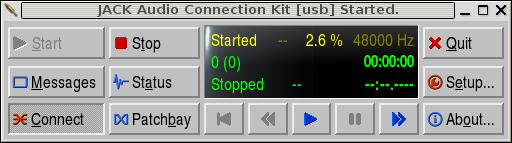
\includegraphics[width=10cm]{image200602/qjackctl-1.png}

詳細の設定を指定すると、jackdの起動オプションを細かく指定できます。

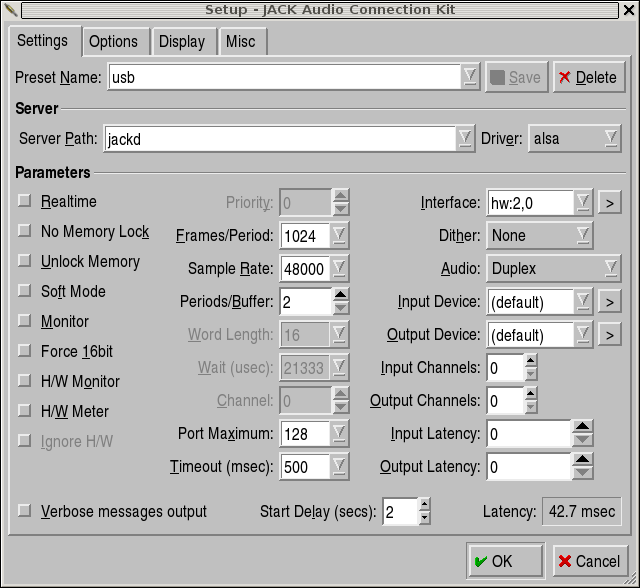
\includegraphics[width=10cm]{image200602/qjackctl-0.png}

また、コネクションパネルを開くと、jack接続の管理が出来ます。

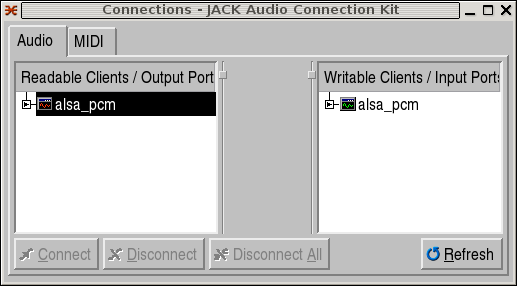
\includegraphics[width=10cm]{image200602/qjackctl-2.png}

\subsubsection{ladspa}

オーディオのエフェクトを処理するための、プラグインインタフェースです。
また、ladspa-devパッケージが存在しており、そのパッケージに含まれている
/usr/include/ladspa.h を利用することが推奨されています。
LADSPA自体がポリシーを定義していますが、Debianのladspaパッケージは、
追加で\url{/usr/share/doc/ladspa-sdk/README.Debian}にて定義されている下記のポ
リシーにしたがっています。

\url{/usr/lib/ladspa/}にパッケージが提供するLADSPAプラグインを提供するこ
と。\verb!LADSPA\_PATH! 環境変数が定義されていない場合には、
\url{/usr/local/lib/ladspa:/usr/lib/ladspa}をデフォルトの検索パスとして
利用すること。

\subsubsection{jack-rack}

apt-get install jack-rackでインストールできます。

jack接続経由でLADSPAエフェクトをかけることができ、エフェクトのパラメータ
をGUIで制御できます。

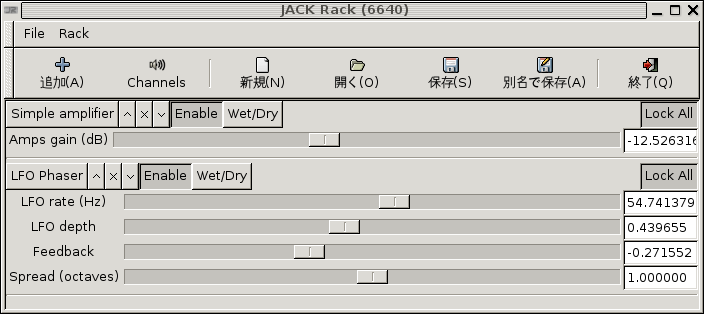
\includegraphics[width=10cm]{image200602/jack-rack.png}

\subsubsection{jamin}

apt-get install jaminでインストールできます。

jack経由で細かいイコライザーやコンプレッサーの設定が出来るツールです。
レコーディングの最終段階のファイナライズに便利そうです。

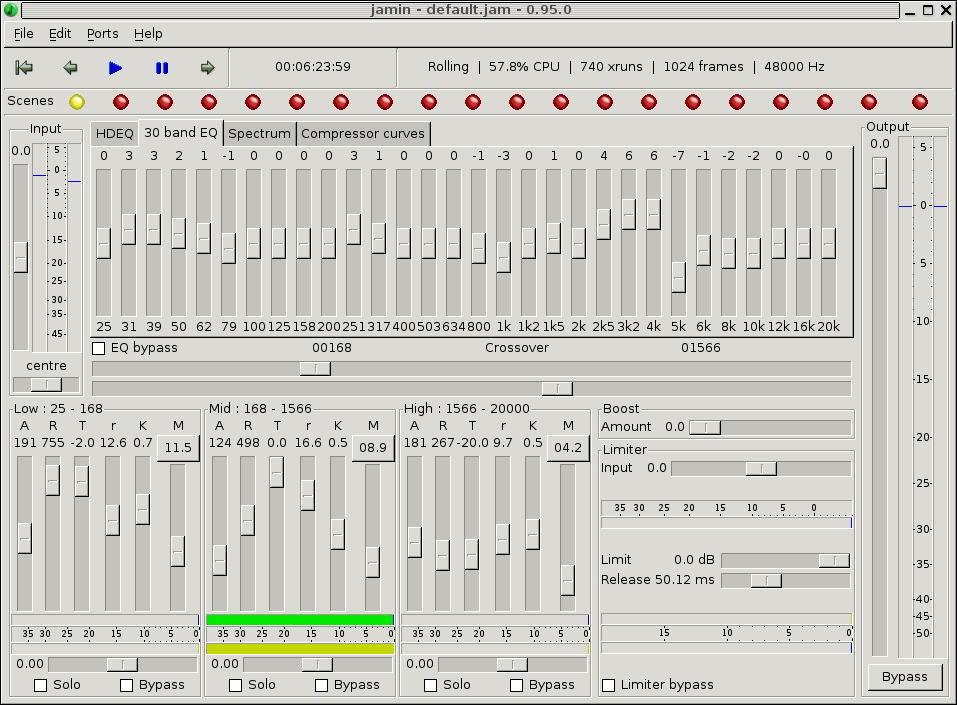
\includegraphics[width=10cm]{image200602/jamin.png}

\subsubsection{jackbeat}

apt-get install jackbeatでインストールできます。wavファイルをリズムルー
プ用のサンプルとして利用して、単純なドラムシーケンサーとして利用できるよ
うです。

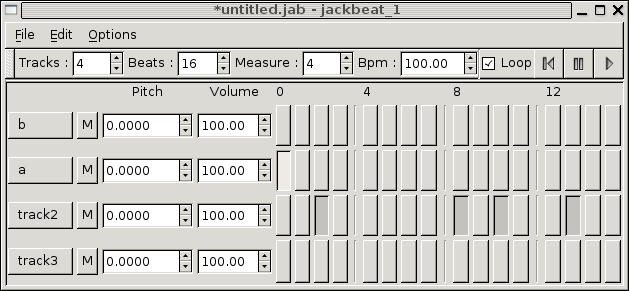
\includegraphics[width=10cm]{image200602/jackbeat.png}

\subsubsection{kluppe}

apt-get install kluppe でインストールできます。
jack経由で接続し、wavファイルをループさせることができます。

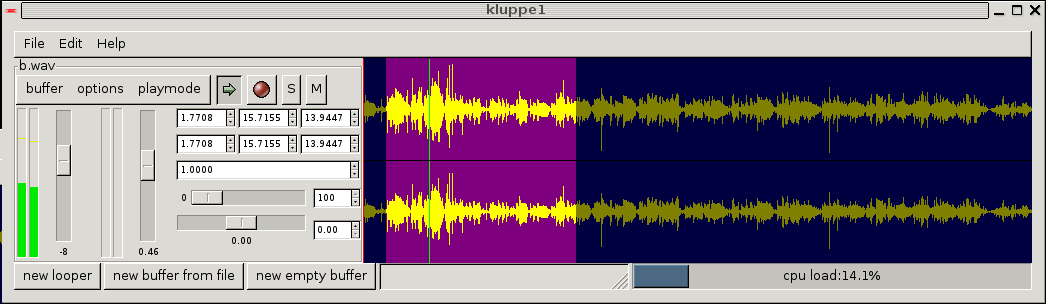
\includegraphics[width=10cm]{image200602/kluppe.png}

\subsubsection{ladcca}

LADCCAというフレームワークが存在しているようです。気づいたらlash
\url{http://www.nongnu.org/lash/} というプロジェクトにかわってしまってい
るようです。セッション管理のためのフレームワークです。jackの導入にともな
い、アプリケーションが接続できるのはよいのですが、毎回アプリケーションを
ユーザが接続する必要があります。その処理を簡便化するためのプロトコルのよ
うです。

\subsection{ソフトウェアシンセ}

MIDIの接続はALSAのMIDI接続が事実上の標準プロトコルとして利用されています。
qjackctl の接続画面にMIDI接続タブがあるので、それを利用して接続してあげればよいです。
また、aconnectというコマンドラインインタフェースがあり、それを利用するこ
とも可能です。

\begin{commandline}
$ aconnect -i -l
クライアント 0: 'System' [タイプ=カーネル]
    0 'Timer           '
    1 'Announce        '
        接続先: 15:0, 128:0
クライアント 14: 'Midi Through' [タイプ=カーネル]
    0 'Midi Through Port-0'
クライアント 130: 'Virtual Keyboard' [タイプ=ユーザ]
    0 'Virtual Keyboard'
        接続先: 129:0
$ aconnect -o -l
クライアント 14: 'Midi Through' [タイプ=カーネル]
    0 'Midi Through Port-0'
クライアント 129: 'FLUID Synth (7910)' [タイプ=ユーザ]
    0 'Synth input port (7910:0)'
        接続元: 130:0
\end{commandline}

\subsubsection{TSE3}

シーケンサエンジンのようです。KDE関連のアプリはこれを利用しているような
気がしています。どうなのよ。

\subsubsection{timidity}

ちょっとインタフェースに古めかしい感がありますが、事実上の標準のMIDIシーケンサエンジンです。MIDIデータからWAVを生成するた
めのインタフェースとして利用されています。

\subsubsection{freepats}

Debianにて、フリーのサウンドフォント集です。形式がpat形式です。timidity
から使える設定になっているようです。

sf2形式じゃないとほとんどのアプリから利用できないので意味が無い。

\subsubsection{zynaddsubfx}

apt-get install zynaddsubfx でインストールできます。

オルガン系の音やパッド系の音が結構使えます。仮想キーボードのUIがお手軽で
す。MIDI制御可能なため、vkeybdを利用して制御することなども可能です。
jack対応です。

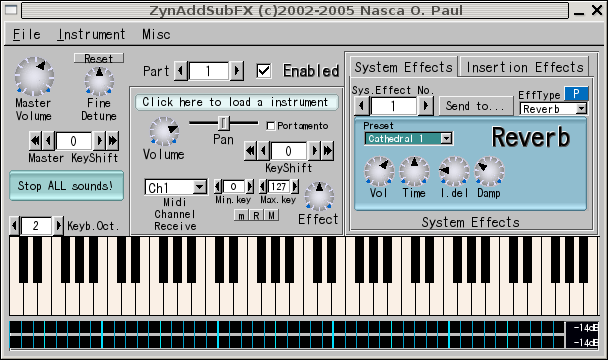
\includegraphics[width=10cm]{image200602/zynaddsubfx.png}

\subsubsection{hydrogen}

UIが優秀なのでドラムシーケンサとして活用しています。
jack 対応です。MIDI入力にも対応しているようです。

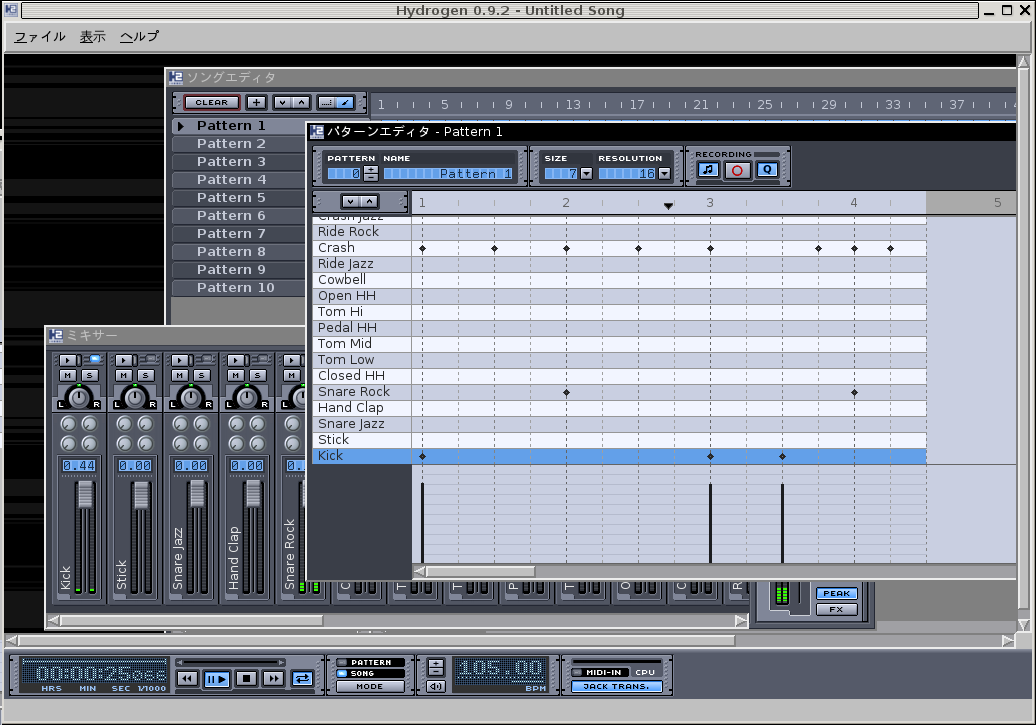
\includegraphics[width=10cm]{image200602/hydrogen.png}

\subsubsection{pd}

UIがかなり前時代的ですが、シンセをGUIで編集するという系では元祖みたいな
存在です。使い方がわからんです。誰か教えてください。

\subsubsection{beast}

GTKシンセ。これも結構頑張っています。使い方がわからんです。誰か教えてください。

\subsubsection{csound}

学術系の人々の中で長い間つかわれてきたものらしく、過去の遺産が大量にあり
ます。ちょっと学術的すぎて個人的には使っていません。誰か使い方教えてくだ
さい。

コマンドラインで操作できる、というよりむしろプログラム言語です。

方程式で波形を設計したいあなたに。

\subsubsection{vkeybd}

キーボードで操作できるMIDIキーボードです。alsaのMIDIデバイスとして動作します。
とりあえず試すのには便利です。
こいつを起動して、qjackctlで接続してあげれば他のアプリケーションがMIDI入
力にどういう反応をするのかを確認できます。

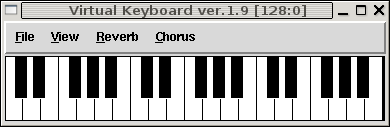
\includegraphics[width=10cm]{image200602/vkeybd.png}

\subsubsection{fluidsynth}

ソフトウェアシンセのようです。sf2形式のファイルをサポートしているようで
す。\url{http://www.hammersound.net/} などに多数のサウンドフォントが存在
していて、そのうちの適当なファイルを読み込んで利用することが出来ます。
jackへ音声を出力することが可能です。

Debian内で、sf2のファイルが見付かりません。
ウェブを探すとたくさんあるようです。

\subsubsection{qsynth}

fluidsynthを制御するGUIです。

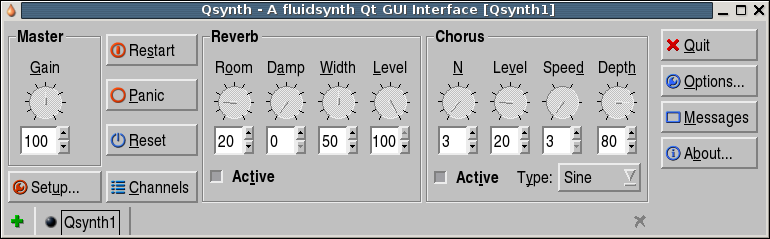
\includegraphics[width=10cm]{image200602/qsynth.png}

\subsubsection{swami}

サウンドフォント(sf2ファイル)を編集するツールです。fluidsynthを内部では
利用しています。

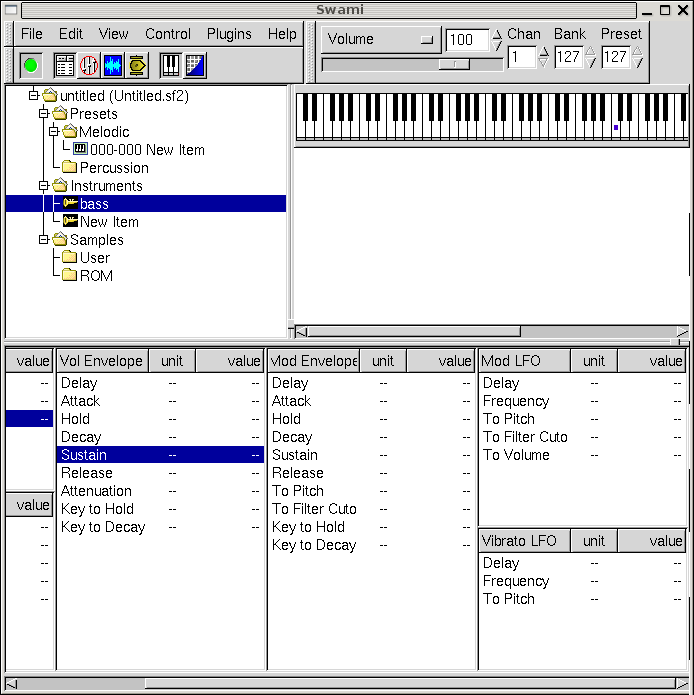
\includegraphics[width=10cm]{image200602/swami.png}

\subsection{楽譜編集}
\subsubsection{lilypond}

\TeX で楽譜を作成しよう、というパッケージ。
まともなクラシックの楽譜を作成するような作業をする際にはこれでやってました。
\TeX をがんがん使いたいあなたに。

\subsubsection{denemo}

今までは上川はこれで一小節程度の楽譜ならこちょこちょっと作成して用を足し
て来ました。キーバインドも数字で音符の長さが決まっていたり、キーの上下で
操作できます。久しぶりに見てみるとインタフェースが大幅に改善されているよ
うです。

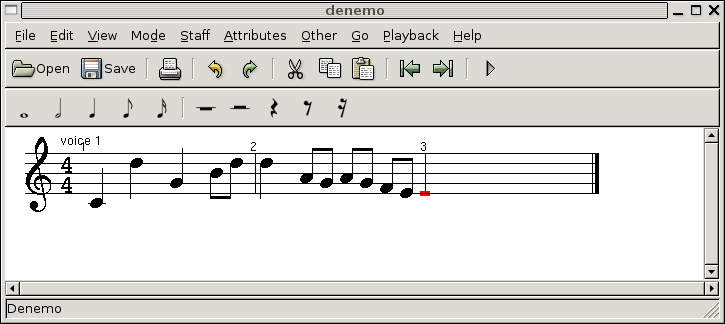
\includegraphics[width=10cm]{image200602/denemo.png}

\subsubsection{noteedit}

MIDIのインポートもできるらしい。
とりあえず楽譜を表示することはできるっぽい。

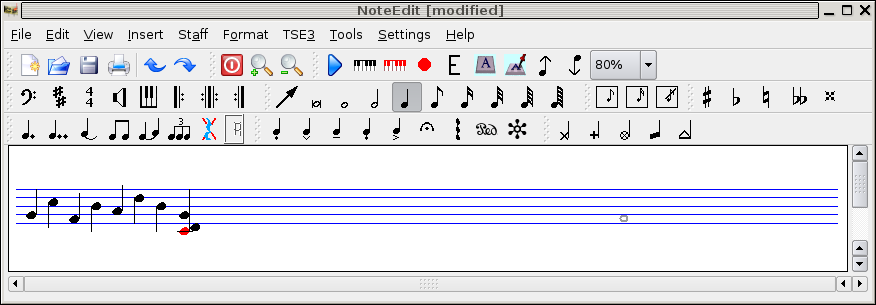
\includegraphics[width=10cm]{image200602/noteedit.png}

\subsubsection{rosegarden4}

apt-get install rosegarden4 でインストール。

一応楽譜が編集できます。ステップ録音などもできます。
デバッグメッセージが大量に出て来るのとなんだか反応が鈍い感じはします。

rosegardenという古くから何度も書き直されつづけているプログラムの最新版で
す。いまのところまともに開発されているようです。

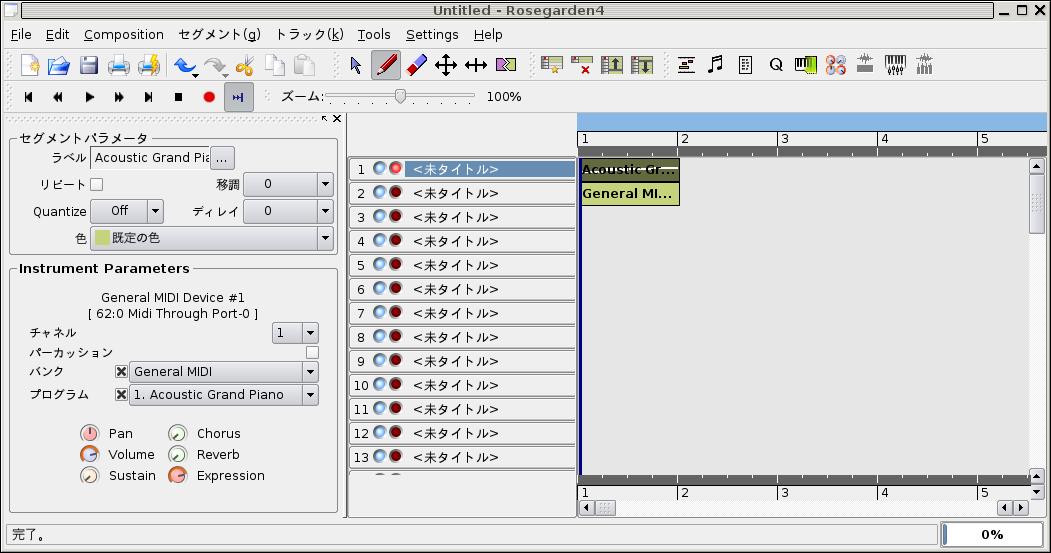
\includegraphics[width=10cm]{image200602/rosegarden4-1.png}

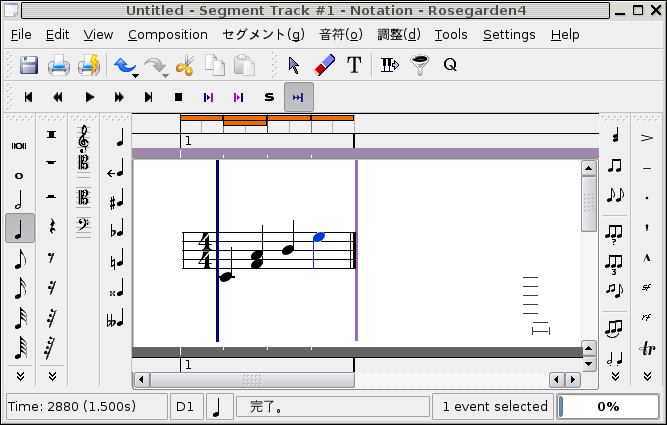
\includegraphics[width=10cm]{image200602/rosegarden4-2.png}

\subsubsection{kguitar}

apt-get install kguitarでインストール。

ギターのタブ譜を編集できるソフトウェアのようです。使い方が分からないので、
困りました。楽譜が出るはずのようですが、出てません。ギターの絵が素敵です。
MIDI入出力ができることになっているようです。

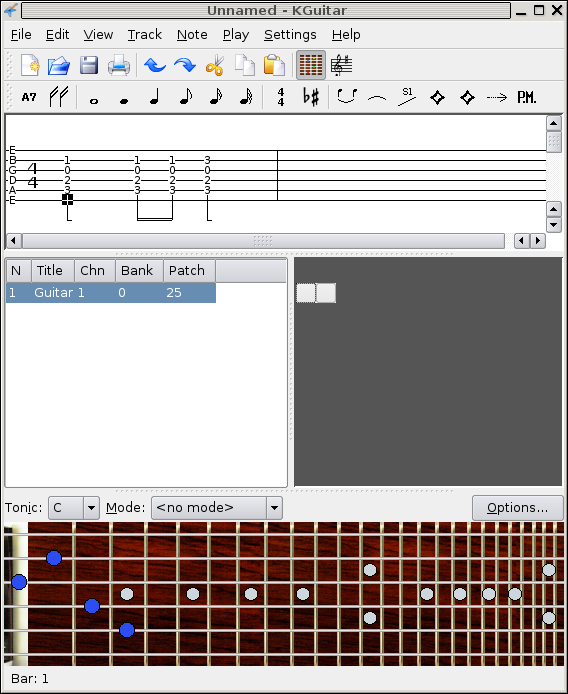
\includegraphics[width=5cm]{image200602/kguitar.png}
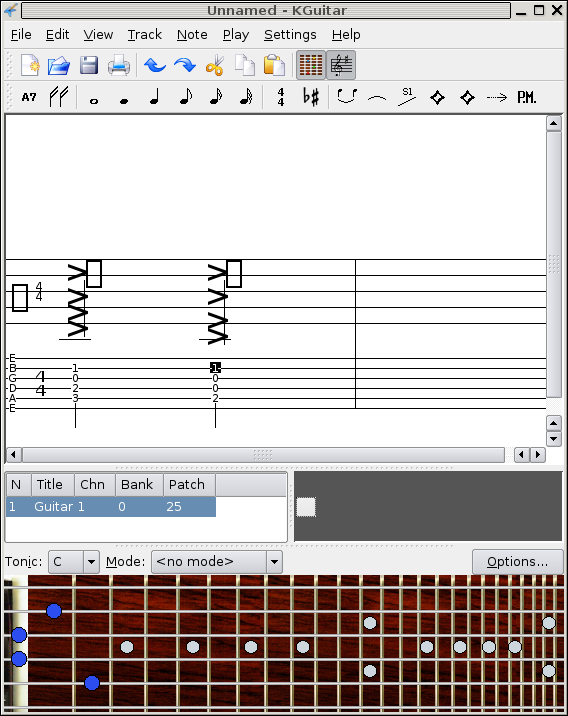
\includegraphics[width=5cm]{image200602/kguitar2.png}

\subsection{音声編集系}

\subsubsection{ecasound}

apt-get install ecasound でインストール。

コマンドラインベースで音声加工をするためのツールです。

よく使うコマンドは

音量をノーマライズする。(可能な最大の音量まであげる)\\
\begin{commandline}
$ ecanormalize in.wav
\end{commandline}
%$

in.wav にコンプレッサーエフェクトをかけて、out.wavを生成する。\\
\begin{commandline}
$ ecasound -i in.wav -o out.wav -eca
\end{commandline}
%$

とりあえず録音する\\
\begin{commandline}
$ ecasound -i alsahw,0,0,0 -o /tmp/a.wav
********************************************************************************
*        ecasound v2.4.3 (C) 1997-2005 Kai Vehmanen and others
********************************************************************************
- [ Session created ] ----------------------------------------------------------
- [ Chainsetup created (cmdline) ] ---------------------------------------------
- [ Connecting chainsetup ] ----------------------------------------------------
(eca-chainsetup) 'rt' buffering mode selected.
(eca-chainsetup) Audio object "alsahw", mode "read".
(audio-io) Format: s16_le, channels 2, srate 44100, interleaved.
(eca-chainsetup) Audio object "/tmp/a.wav", mode "read/write".
(audio-io) Format: s16_le, channels 2, srate 44100, interleaved.
- [ Chainsetup connected ] -----------------------------------------------------
(eca-control-objects) Connected chainsetup: "command-line-setup".
- [ Controller/Starting batch processing ] -------------------------------------
- [ Engine init - Driver start ] -----------------------------------------------

ここでctrl-Cで停止

- [ Controller/Processing stopped (cond) ] -------------------------------------
- [ Engine exiting ] -----------------------------------------------------------
(eca-control-objects) Disconnecting chainsetup: "command-line-setup".
- [ Chainsetup disconnected ] --------------------------------------------------
- [ Controller/Batch processing finished ] -------------------------------------
\end{commandline}
%$


\subsubsection{sweep}

apt-get install sweep でインストール。

メモリ上にwavファイルを展開するので、大きいwavファイルは編集できないです。
プリビューが優秀。ダブルクリックしたらそこから再生したりしてくれる。
こまかい波形の切りだしなどに上川愛用。
しかし、jackに対応していないなどの欠点があります。

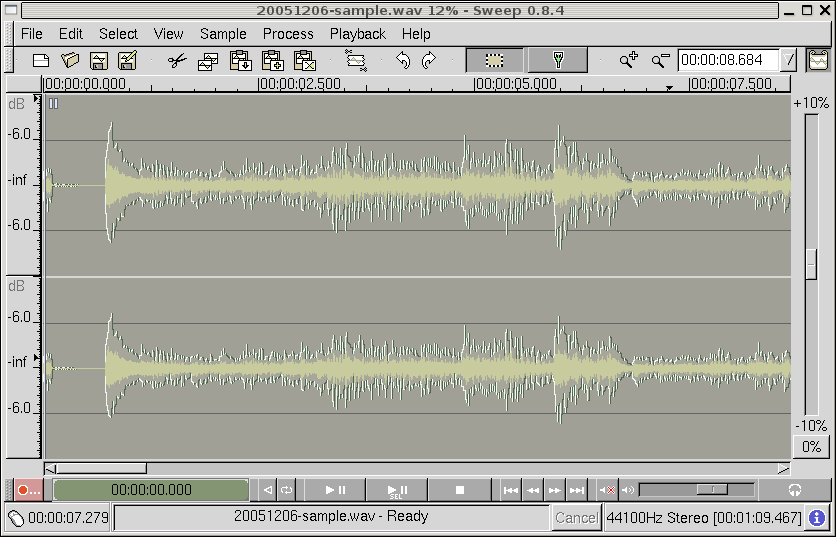
\includegraphics[width=10cm]{image200602/sweep.png}

\subsubsection{rezound}

apt-get install rezound でインストール。

サウンドの編集用のツールです。jack出力をサポートしています。

\begin{commandline}
$ rezound --audio-method jack
\end{commandline}

録音を開始する場合にはデバイスを確認されます。

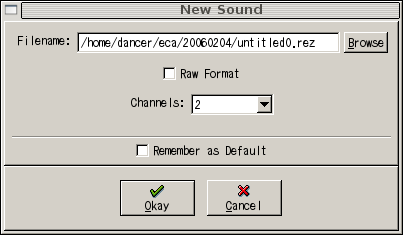
\includegraphics[width=5cm]{image200602/rezound-1.png}
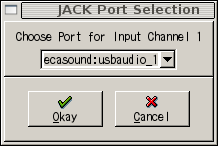
\includegraphics[width=3cm]{image200602/rezound-2.png}
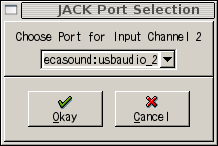
\includegraphics[width=3cm]{image200602/rezound-3.png}

録音する際にはレベルの表示もしてくれます。

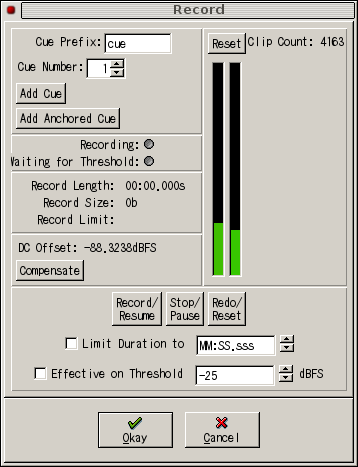
\includegraphics[width=5cm]{image200602/rezound-4.png}

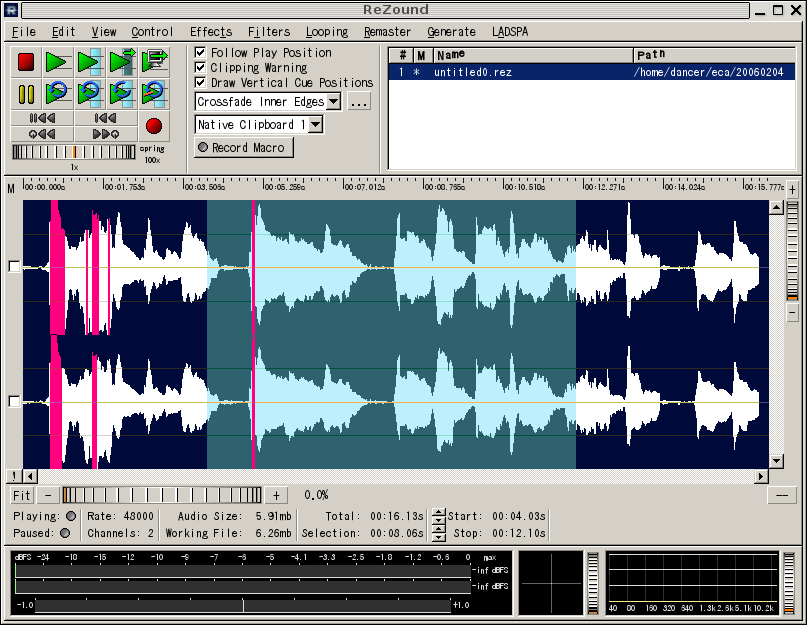
\includegraphics[width=10cm]{image200602/rezound-5.png}

入出力はjackで設定してあげます。

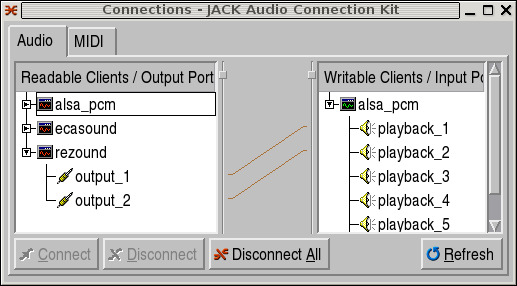
\includegraphics[width=6cm]{image200602/rezound-6.png}

\subsubsection{audacity}

apt-get install audacity でインストール。

audacityで起動。マルチトラックのオーディオ編集に最適。巨大な波形データも
メモリ上に全てをロードしようとはしないので編集できる。巨大なデータの一次
処理用には上川愛用。しかし、jackをサポートしていません。

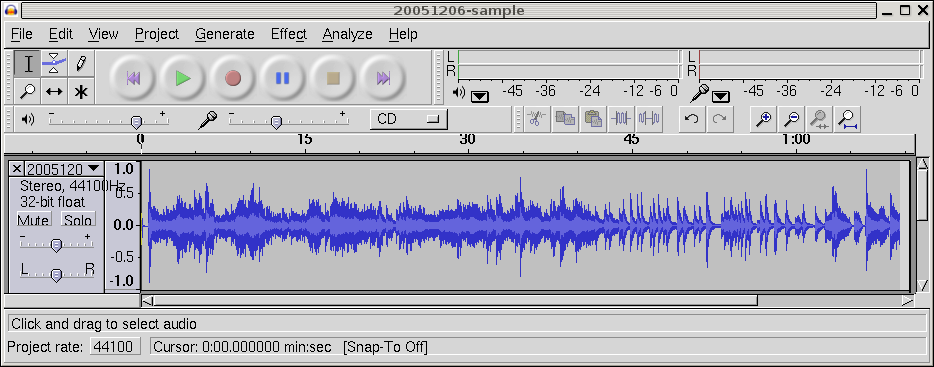
\includegraphics[width=10cm]{image200602/audacity.png}

以前は日本語インタフェースを利用しようとすると悲惨でしたが、直っているよ
うです。まだ一部問題が残っているようですが、全く使えないほどではないです。

\subsubsection{ardour}

apt-get install ardour-gtk でインストール。

マルチトラックの音声ファイルは編集できるけど、音符が編集できそうな雰囲気
は無いです。

Paul Davisという人が中心に開発していて、彼はこのためにjackとLADSPAを実装
し、Hammerfall のサウンドカードのドライバをALSA用に実装したというよくわ
からないけど凄い代物です。

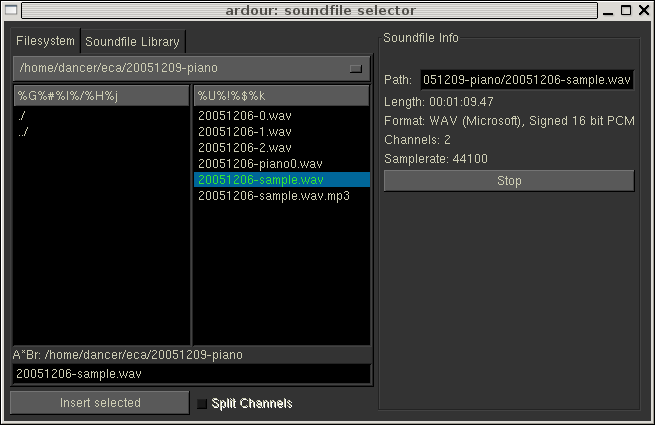
\includegraphics[width=10cm]{image200602/ardour1.png}

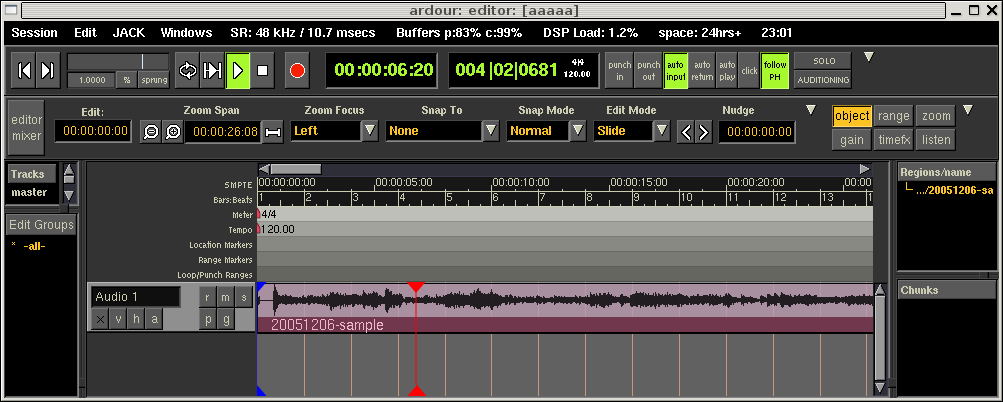
\includegraphics[width=10cm]{image200602/ardour2.png}

\subsubsection{muse}

apt-get install muse でインストール。

MIDIトラックと音声トラックが同時に扱えるようです。jackとALSA MIDIに対応
しているようです。使い方がわからず。

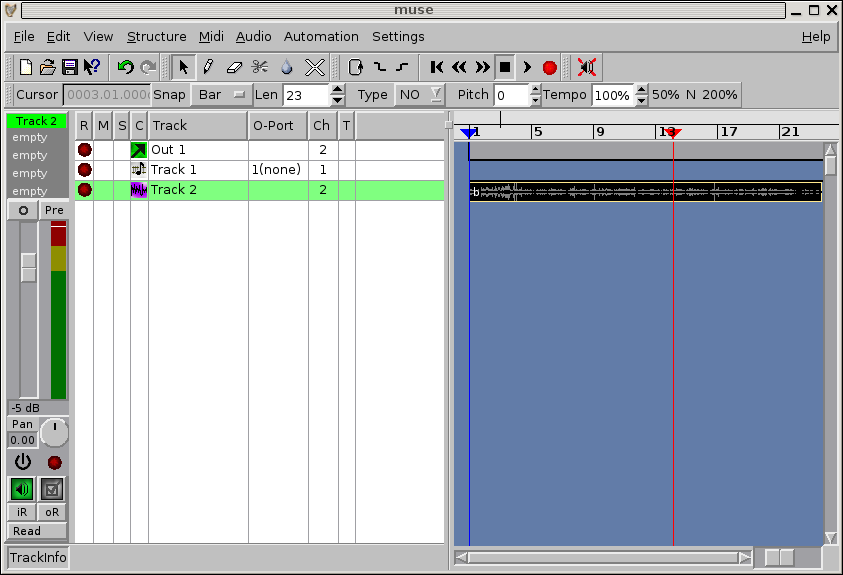
\includegraphics[width=10cm]{image200602/muse.png}


\subsubsection{snd}

音声業界でのemacsと呼ばれています。使い方がわからないです。誰か教えて下
さい。

\dancersection{次回}{}

3月はオープンソースカンファレンスにお邪魔する予定です。
内容は本日決定予定です。

参加者募集はまた後程。

\newpage

\vspace*{15cm}
\hrule
\vspace{2mm}

\includegraphics[width=2cm]{image200502/openlogo-nd.eps}
\noindent \Large \bf Debian 勉強会資料\\ \\
\noindent \normalfont 2006年2月18日 \hspace{5mm}  初版第1刷発行\\
\noindent \normalfont 東京エリア Debian 勉強会 (編集・印刷・発行)\\
\hrule

\end{document}
